%*----------- SLIDE -------------------------------------------------------------
\begin{frame}[t]{Introdução} 
    \transdissolve[duration=0.5]
    Este mini curso é oferecido pelo Laboratório de Robótica e Sistemas Autônomos (RoSA) do SENAI CIMATEC.

    \begin{columns}[t]
        \column{.5\linewidth}
          \begin{center}
            %\centerline{
                \begin{figure}
                    %
\includegraphics[width=1\textwidth]{pista}
                    % \caption{Pista de corrida \cite{agostini2007}}
                    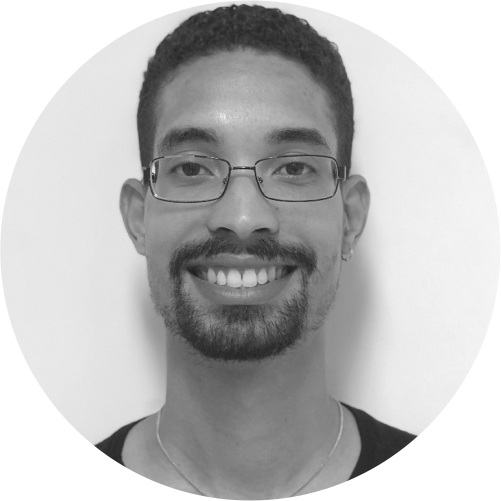
\includegraphics[width=.55\linewidth]{leo.png}
                    \caption{Leonardo Lima}
                    %\caption{Pista de corrida \cite{agostini2007}}
                \end{figure}
            %}
            \end{center}            

        \column{.5\linewidth}
        \begin{center}
        %\centerline{
            \begin{figure}
                %
\includegraphics[width=1\textwidth]{pista}
                % \caption{Pista de corrida \cite{agostini2007}}
                
\includegraphics[width=.55\linewidth]{felipe.png}
                \caption{Felipe Mohr}
                %\caption{Pista de corrida \cite{agostini2007}}
            \end{figure}
        %}
        \end{center}
    \end{columns}
\end{frame}

%*----------- SLIDE -------------------------------------------------------------
\begin{frame}[t]{O que é Robótica Móvel?}
  \transboxout[duration=0.5]
  Robôs móveis são robôs dotados de um sistema de locomoção que os torna capazes de navegar através do seu ambiente de trabalho \cite{robmovel}.

  % \framesubtitle{Darwin-OP}
  \begin{columns}[c]
    \column{.33\textwidth}
      \begin{center}
        \begin{figure}
          \includegraphics[width=.9\textwidth]{mob1.png}  
        \end{figure}
      \end{center}      
    \column{.33\textwidth}
      \begin{center}
        \begin{figure}
          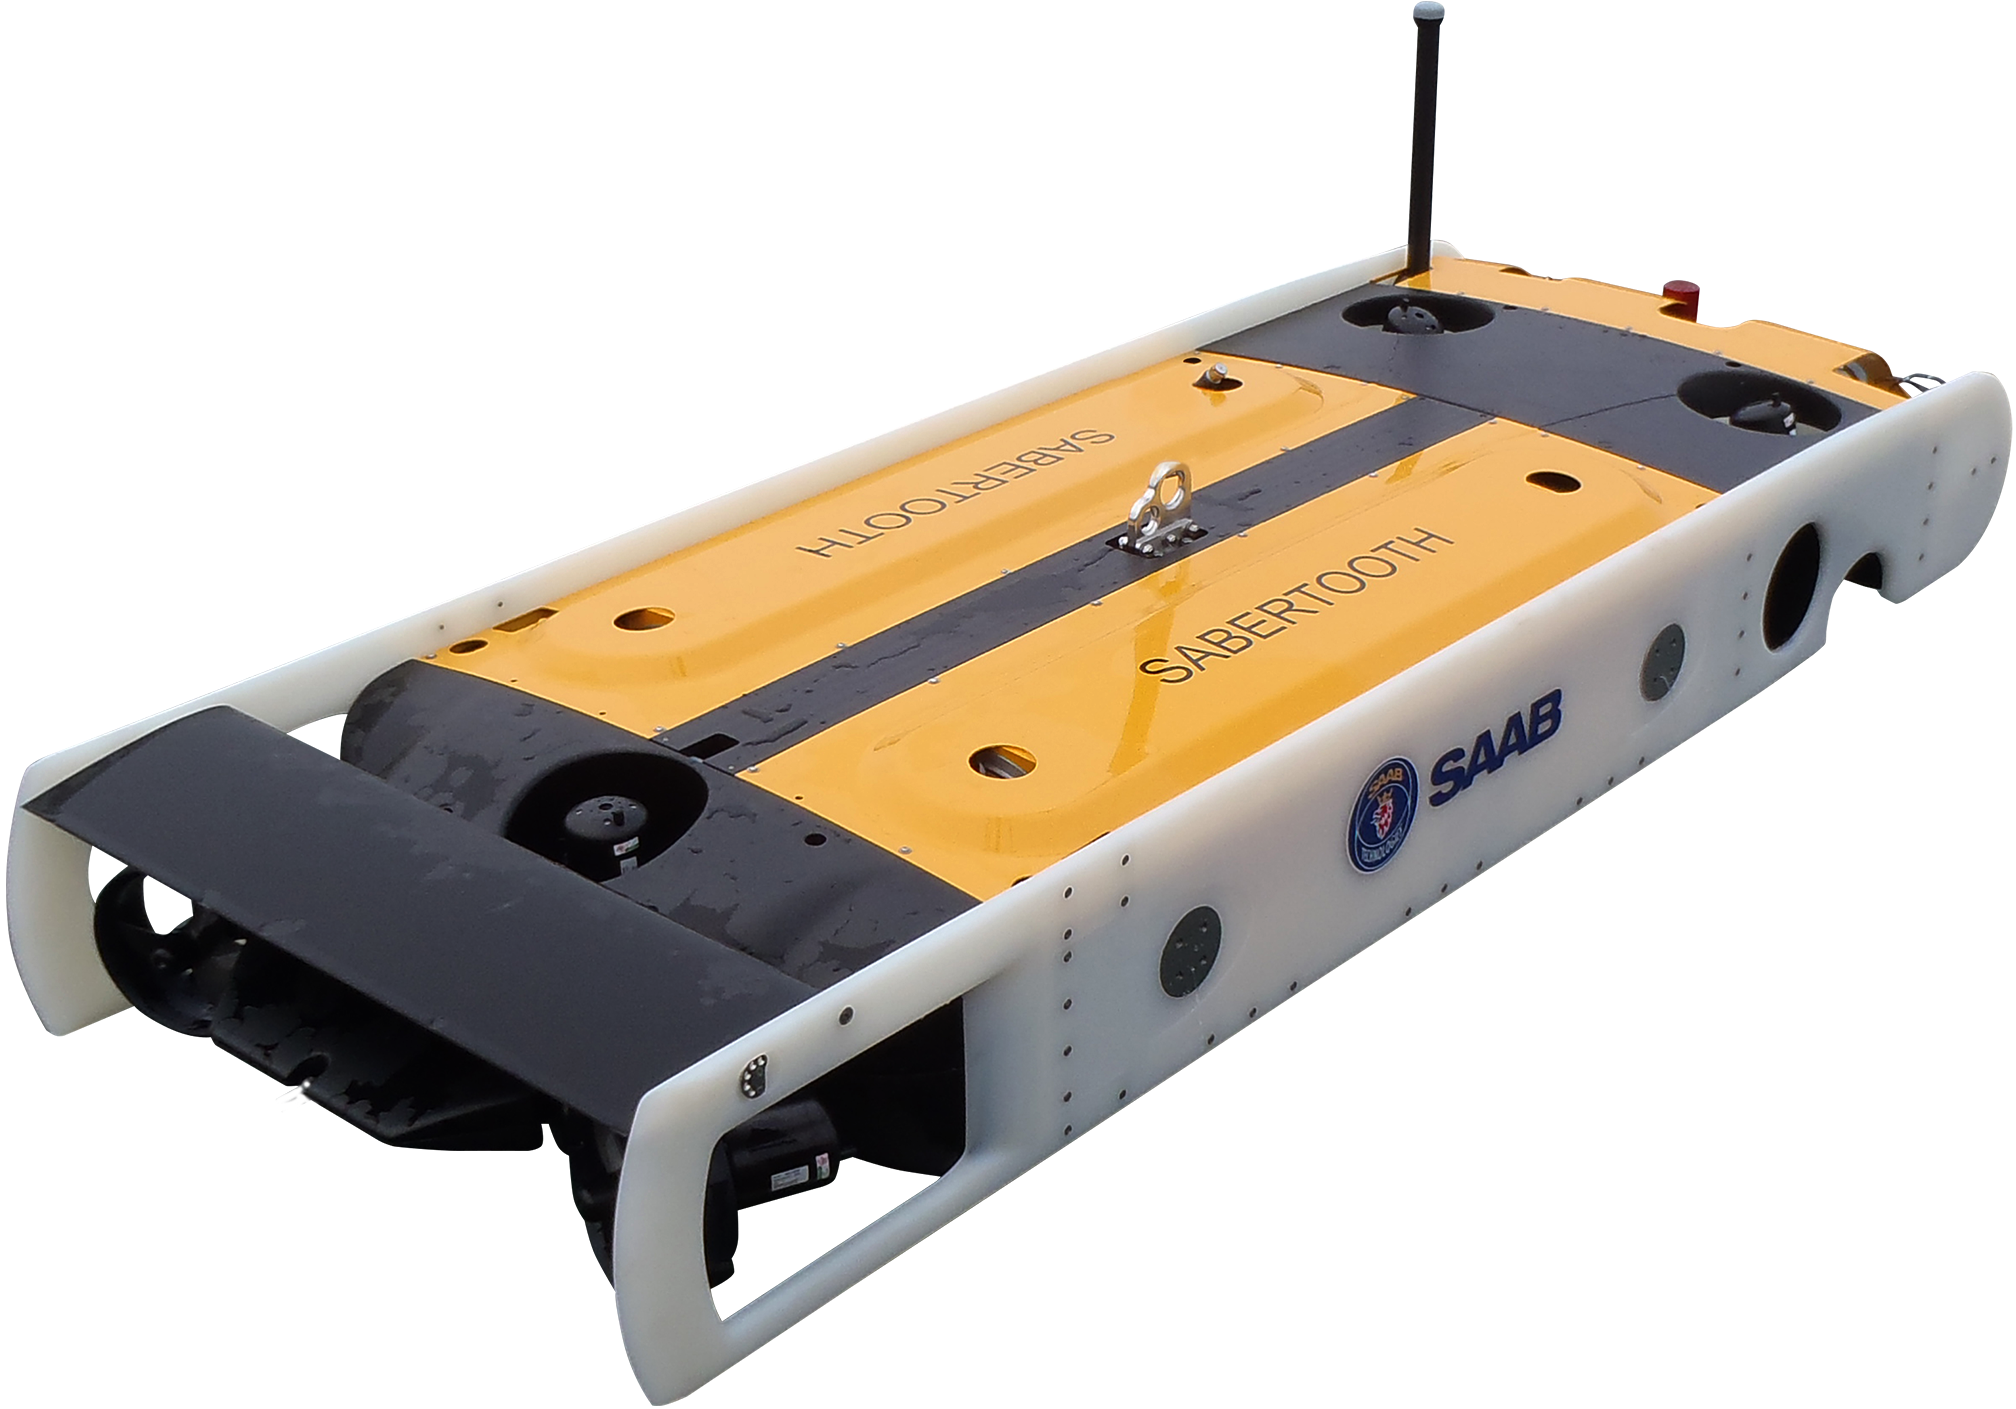
\includegraphics[width=.9\textwidth]{mob2.png}  
        \end{figure}
      \end{center}      
    \column{.33\textwidth}
      \begin{center}
        \begin{figure}
          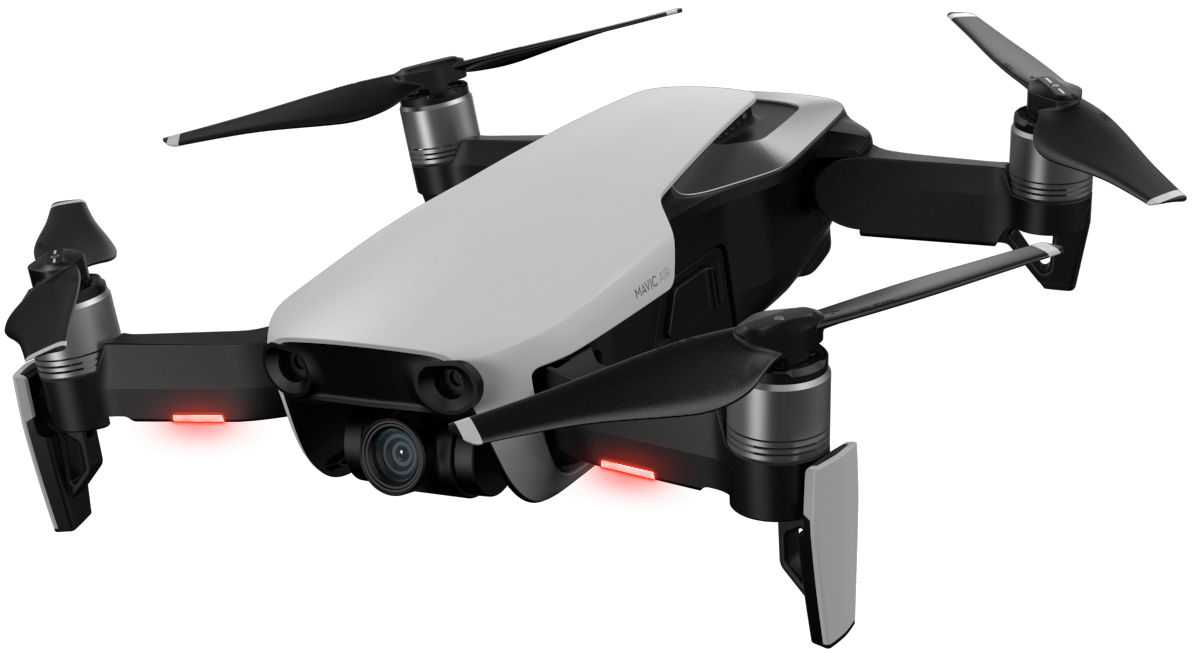
\includegraphics[width=.9\textwidth]{mob3.png}  
        \end{figure}
      \end{center}
  \end{columns}
\end{frame}

%*----------- SLIDE -------------------------------------------------------------
\begin{frame}
  \begin{center}
    \begin{figure}
      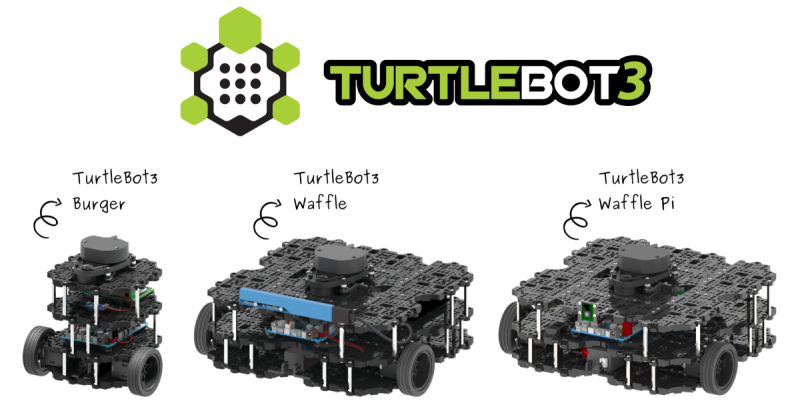
\includegraphics[width=1.0\textwidth]{turtlebot3.png}  
    \end{figure}
  \end{center}
\end{frame}